\chapter{Introduction}
\label{Chapter1}

\section {Genetic variation in humans }

No human is genetically the same as another, any two humans differ, on average, at about 1 in 1,000 DNA base pairs (0.1\%).
Over the past 20 years, the study of genetic variation in human has increased exponentially with an explosion of human genetic data. 
Innumerable DNA sequences and genotypes have been generated, and they have led to significant biomedical advances. 
In 2001 the whole genome reference sequence of humans was made publicly available to the scientific community  providing the first comprehensive description of the human genome (\cite{lander2001initial})

The first large-scale project that made use of whole-genome sequencing was the 1000 genomes project that used a combination of low-coverage whole-genome sequencing (WGS), deep exome sequencing, and dense microarray of 2,504 individuals from 26 populations. 
This project showed that two individuals differ at roughly  0.6\% of their genome, that corresponds at 20 millions base pairs at 4.1-5.0 million sites in a genome of 3.2 giga base (\cite{1000genome2015global}). \\

A more recent study identifies 67.3 million single-nucleotide polymorphisms, 8.8 million small insertions or deletions (indels), and 40,736 copy number variants in 929 genomes from 54 geographically diverse human populations, the technology used was high-coverage whole-genome sequencing at 35X coverage (\cite{bergstrom2020insights}). 
The number of variants identified by this study is comparable to the one identified by the 1000 genome project (84.7 million SNPs discovered in 2,504 individuals) despite the lower sample size because the high-coverage sequencing increased the sensitivity. Furthermore, this study also identified 1.3 million polymorphic SNPs shared between archaic human genomes. (Figure \ref{fig:HGDP}) \\

\begin{figure}[H]
\centering
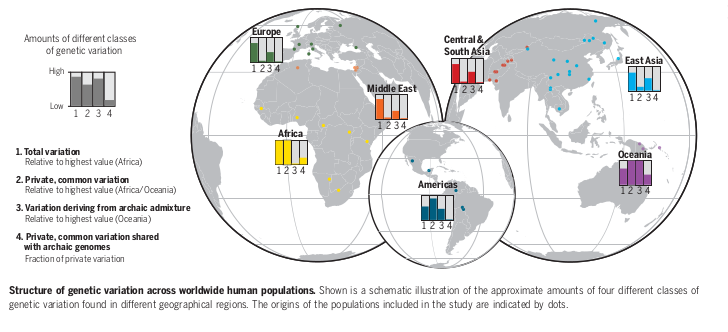
\includegraphics[width=1\textwidth]{Fig/HGDP.png}
\decoRule
\caption{}
\label{fig:HGDP}
\end{figure}

\section{Mitochondrial Genomes}
\subsection{Structure and function of mitochodria}
Mitochondria are a membrane-bound organelle present in the cytoplasm of all eukaryotic cells. They are responsible for producing Adenosine triphosphate (ATP), the main energy currency of the cell.
Mitochondria are typically round to oval in shape and range in size from 0.5 to 10 $\mu$m. In addition to producing energy, mitochondria store calcium for cell signaling activities, generate heat, and mediate cell growth and death.
Mitochondria are unlike other cellular o.<rganelles in that they have two distinct membranes and a unique genome and reproduce by binary fission. 
The outer mitochondrial membrane is freely permeable to small molecules and contains special channels capable of transporting large molecules. 
In contrast, the inner membrane is far less permeable, allowing only very small molecules to cross into the gel-like matrix that makes up the organelle’s central mass. 
The matrix contains the DNA of the mitochondrial genome (mtDNA) and the enzymes of the tricarboxylic acid (TCA) cycle (also known as the Krebs cycle), which metabolizes nutrients into by-products the mitochondrion can use for energy production. (Figure \ref{fig:Mitochondrial Function}) (\cite{friedman2014mitochondrial})

\subsection{Mitochondrial genome}
Mitochondrial DNA (mtDNA) is a double-stranded molecule of 16.6 kb. The two strands of mtDNA differ in their base composition, with one being rich in guanines, making it possible to separate a heavy (H) and a light (L) strand. The mtDNA contains one longer noncoding region (NCR) also referred to as the control region. DNA polymerase γ (POLγ) is the replicative polymerase in mitochondria. 
The circular genome contains 13 protein‐encoding sequences corresponding to subunits ND1‐6, including ND4 and ND4L, of respiratory complex I, catalytic subunits cytochrome c oxidase subunit I-III (CO1-3) of respiratory complex IV, subunits adenosine triphos-phate 6 (ATP6) and ATP8 of F1F0 ATPase, and cytochrome B of respiratory complex III. 
The remaining genes encode 22 tRNAs and 12, and 16S rRNAs. (Figure \ref{fig:Mitochondrial Genome}, \cite{stefano2016mitochondrial, garone2018mitochondrial})\\

Each human cell contains thousands of copies of mtDNA. At birth these are usually all identical (homoplasmy). Through life mutations can occur in one mtDNA and its descendants creating genetic variability of mitochondrial DNA within the same cell (heteroplasmy). Some of these mutations might be deleterious, therefore individuals with mitochondrial disorders resulting from mutation of mtDNA may harbor a mixture of mutated and wild type mtDNA within each cell. 

In many organisms, the mitochondrial genome is inherited maternally. This is because the mother’s egg cell donates the majority of cytoplasm to the embryo, and mitochondria inherited from the father’s sperm are usually destroyed but paternal mitochondrial DNA (mtDNA) transmission may coexist with maternal transmission of mtDNA. In a study on a family with mitochondrial disorders it was found that there was a high level of heteroplasmy due to paternally transmission (\cite{luo2018biparental}). 

\begin{figure}[H]
\centering
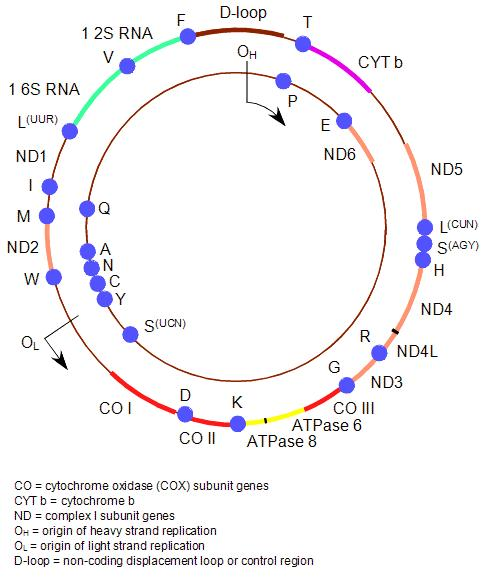
\includegraphics[width=0.7\textwidth]{Fig/mitogenome.jpg}
\decoRule
\caption{\textbf{Mitochondrial Genome}}
\label{fig:Mitochondrial Genome}
\end{figure}

\begin{figure}[H]
\centering
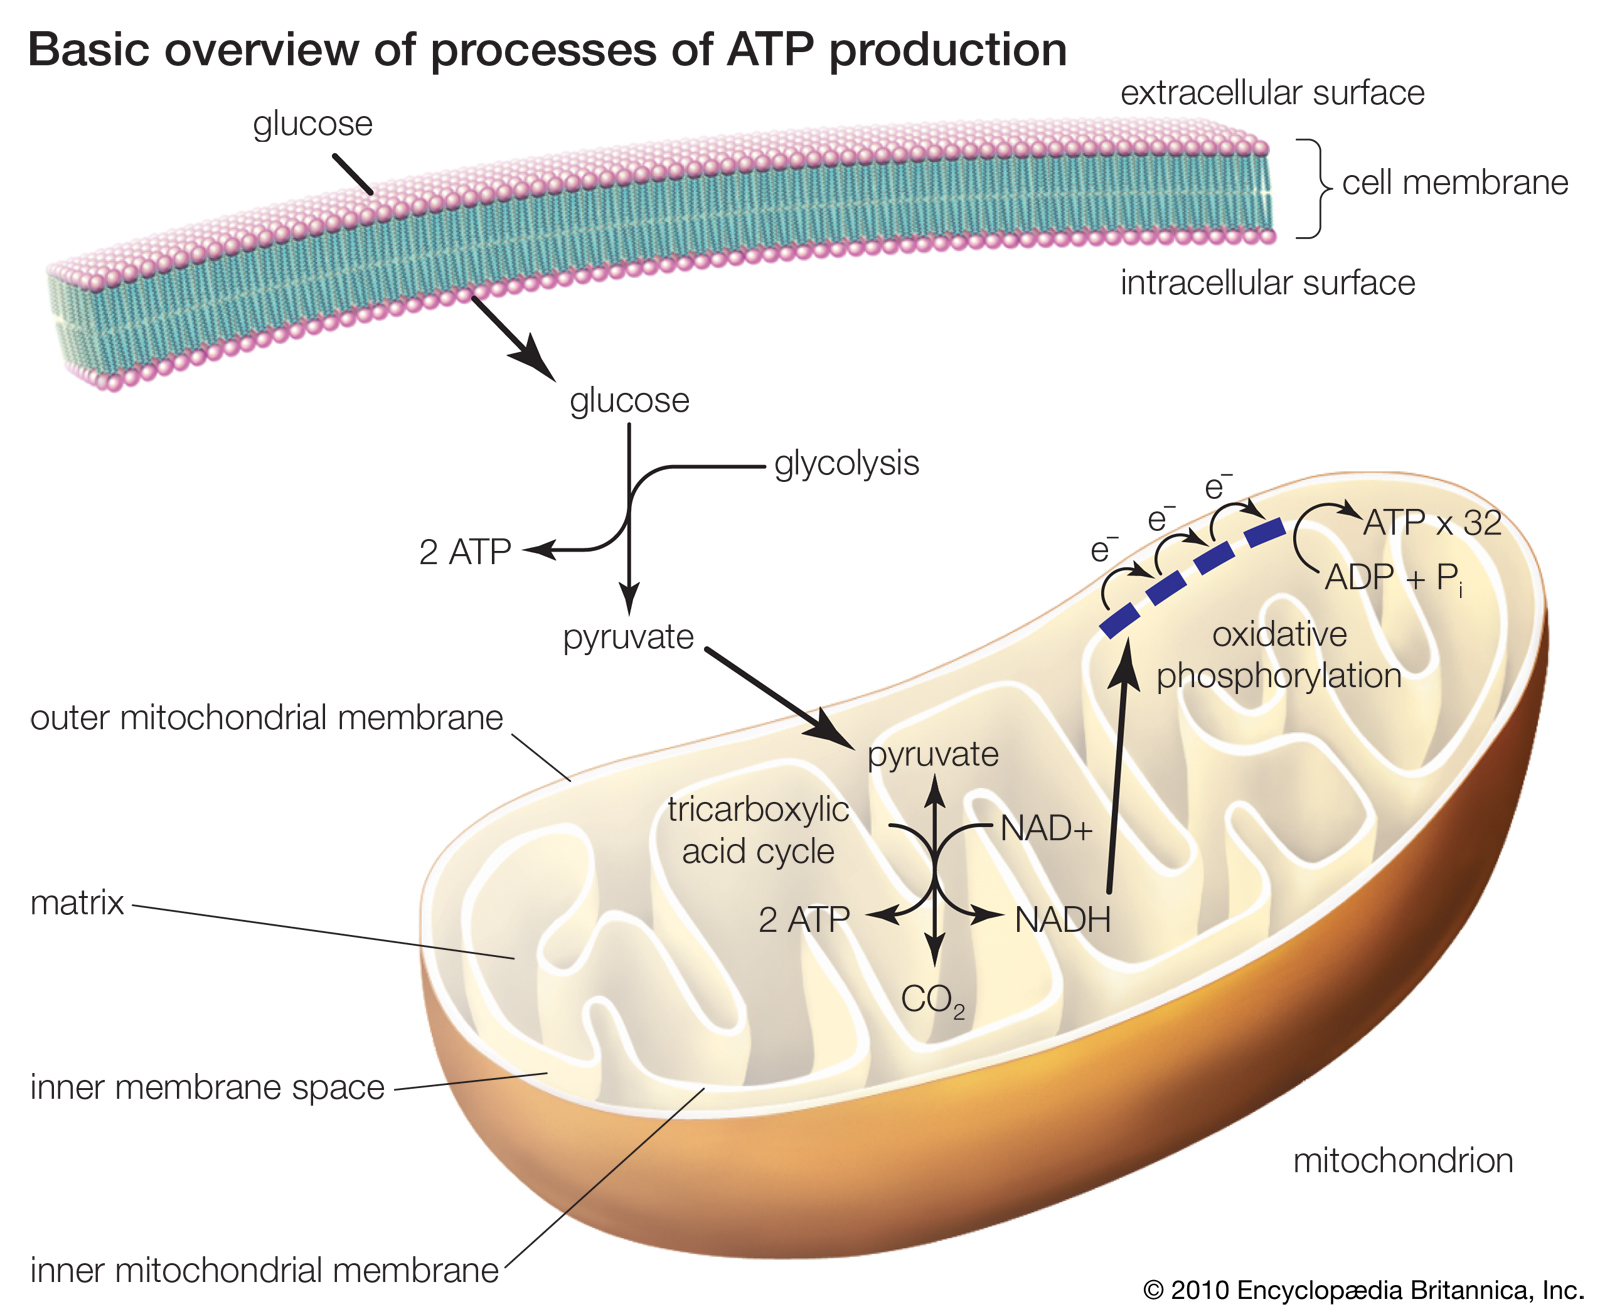
\includegraphics[width=0.7\textwidth]{Fig/processes-production-ATP-glycolysis-tricarboxylic-acid-cycle.jpg}
\decoRule
\caption{\textbf{Mitochondrial Function}}
\label{fig:Mitochondrial Function}
\end{figure}


\newline

\section{Expression of nuclear genes product in the mitochondria}
Not all the process taking place in mitochondria are controlled by mtDNA, in fact more than 1000 nuclear genes encode mitochondrial proteins.
Important mitochondrial mechanisms controlled by nuclear genes include disorders of mtDNA maintenance (mtDNA depletion or secondary pathogenic mtDNA variants), enzymes for lipid or cofactor biosynthesis (\textit{TAZ}), genes encoding factors for mitochondrial protein synthesis like the mitoribosomes encoded by \textit{MRPS22} (\cite{caggese1999identification, chinnery2014mitochondrial}). 
Most nuclear genes encode factors involved in the assembly of the complexes of the respiratory chain, like \textit{COX} genes, involved in stability and assembly of the respiratory complex.


\section{Mitochondrial Diseases}
Mitochondrial diseases are a clinically heterogeneous group of disorders that arise as a result of dysfunction of
the mitochondrial respiratory chain.
Single-cell studies and cybrid-cell studies have shown that the proportion of mutated mtDNA must exceed a critical threshold level before a cell expresses a biochemical abnormality of the mitochondrial respiratory chain (the threshold effect). The percentage level of mutated mtDNA may vary among individuals within the same family, and also among organs and tissues within the same individual (\cite{chinnery2014mitochondrial, thorburn2017mitochondrial}). 
While some mitochondrial disorders only affect a single organ (for example the eye in Leber hereditary optic neuropathy LHON), many involve multiple organ systems and often present with prominent neurologic and myopathic features , like Leigh syndrome.
Leigh syndrome (also called Leigh disease or subacute necrotizing
encephalomyelopathy) is a rare inherited neurometabolic disorder
and affects the central nervous system. 
Genetically, alterations or mutations of the mitochondrial respiratory enzyme complex or pyruvate dehydrogenase complex are believed to be responsible for the development of Leigh syndrome.
Brainstem dysfunction manifests as respiratory symptoms and abnormalities in swallowing, ophthalmology, and thermoregulation. 
The neurologic manifestations may begin in infancy or early
childhood, progressively worsen, and eventually lead to death in
early childhood ; Leigh syndrome can also occur at any age, including adolescence or adulthood.
(\cite{chang2020meta})


\section{Genetic causes of miscarriages}
Inefficiency in reproductive processes is known in humans. The prevalence of a miscarriage has been estimated to be between 10 and 15\% of all pregnancies, with the majority of these occurring in the first trimester of pregnancy.
Miscarriage is defined as the spontaneous termination of a pregnancy before 24 weeks of gestation.(\cite{larsen2013new , goddijn2000genetic}).
Miscarriages can occur for medicals or genetics causes. The most common medicals causes are TORCH infections, hypothyroidism,  diabetes and  uterine  anatomical  abnormalities . (\cite{najafi2019chromosomal}) . Among the genetic causes, chromosomal abnormalities are the major factor underlying early miscarriage and the most common are chromosomal aneuploidies such as trisomies or deletions of large chromosomal chunks (\cite{zhang2009genetic}) and can occur during mitosis in the oocytes or in sperms. Miscarriages can also have non random genetic causes like small mutations (SNPs and indels), both de-novo or inherited from parents (\cite{larsen2013new}).

\subsection{Mitochondrial diseases in miscarriages}

As far as genetic causes are concerned, it is important to remember the contribution of mitochondrial DNA in human reproduction inefficiency. 
Structural, spatial and genetic dysfunctions that affect the capacity of mitochondria to produce ATP by oxidative phosphorylation could have pleiotropic affects on early human development that may include the normality of spindle organization and chromosomal segregation. Mitochondrial dysfunctions that contribute to the activation of apoptosis may be a cause of human oocyte wastage and early embryo demise (\cite{van2004mitochondria}).
Mitochondrial dysfunction in the oocyte may be a critical determinant of the developmental competence of an early human embryo. Mitochondrial dysfunctions affecting ATP production during early developmental stages may be lethal for the embryo, even if only a portion of the mitochondria are dysfunctioning (\cite{karaa2019effects ,kaare2009mitochondrial}). Consequently, it is possible that some mtDNA mutations cause developmental arrest already before the pregnancy is clinically recognized (\cite{van2004mitochondria}). A fundamental role in mitochondrial diseases is played by homoplasmy/heteroplasmy level.
Homoplasmy for a severe pathogenic mtDNA mutation is rarely observed, presumably because of embryo lethality. 
Although a homoplasmic tRNA mutation has been reported in a family with six neonatal deaths and a miscarriage (\cite{mcfarland2002multiple}), mitochondrial mutations for diseases such as mitochondrial encephalopathy with lactic acidosis and stroke-like episodes (MELAS) and myoclonic epilepsy and ragged-red fibers (MERRF) are heteroplasmic, and homoplasmic mutations causing these syndromes would probably cause fetal demise (\cite{van2004mitochondria}).


\section{Project GREP}
The work I have done during my thesis is part of the project \textit{Genomics of REcurrent Pregnancy loss (GREP)} lead by the Institute of Genetics and Biophysics of the National Research Council in collaboration with the University of Napoli Federico II, and several other partners in Italy, United Kingdom, Malaysia, Pakistan, and Australia.  

GREP aims to identify genetic variants likely to cause PL not seen by current diagnostic tools (mainly comparative genomic hybridization), either because of the size or because they are located in non-coding regions not considered in medical diagnostics. The main objective of GREP is to build a predictive model that integrates genomic variation and functional annotations, based on the analysis of whole-genome sequences of miscarried embryos.\\

\chapter{Aim of the thesis }
%prima parte tesi gianluca
I participate in the data analyses of the GREP pilot project that includes four main stages (Figure \ref{fig:projectPhases}). The first step was the collection of samples done by the University of Ferrara during 2016-2018, followed by a step of screening for euploid samples to be sequenced. Sequenced samples are being analyzed and the results will be validated using a biobank of embryonic DNA and eventually cellular models.\\

The main part of my thesis is the study and analysis of mitochondrial DNA. In particular I analyzed the mitochondrial genome of ten embryos from recurrent miscarriages In order to characterize mitochondrial genetic variability (Homoplasmy and Heteroplasmy) to have a broad spectrum of the mitochondrial genome and its characteristics such as to be able to identify potentially detrimental variants and the genes potentially involved in mitochondrial diseases and miscarriages.
Furthermore, I determined the haplogroups of the ten samples in order to deepen the analyses.


\begin{figure}[H]
\centering
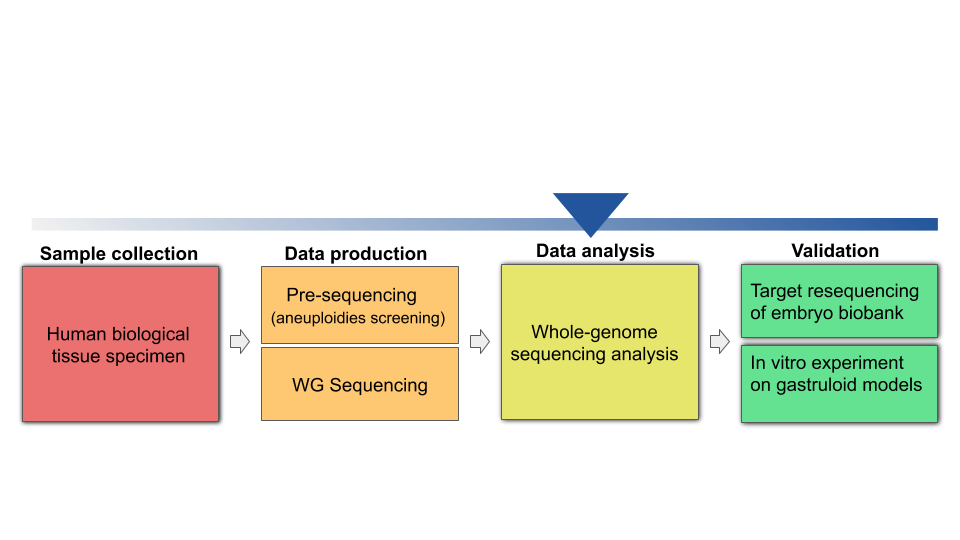
\includegraphics[width=0.80\textwidth]{Fig/projectPhases.png}
\decoRule
\caption{\textbf{Pilot project phases.}} 
\label{fig:projectPhases}
\end{figure}







